\newpage
\chapter{Trade-Off Method \& Criteria}
\label{ch4-method}

This chapter will focus on explaining how the trade-off will be performed to select a winner from our various concepts. The criteria that will be used in trading off the concepts will be introduced. For this, both quantitative and qualitative criteria are discussed. Also, the method to weigh the various criteria is explained in \autoref{subsec:weights}. 

\section{Criteria}
\label{sec:Criteria}
%Should we separate between qualitative and quantitative criteria?

In order to choose a final concept to further develop during the detailed design phase, a set of criteria must be established to compare the candidate concepts. The criteria, along with the weights associated with each criterion heavily affect the concept that gets chosen in the trade-off. Given that the criteria will drive the solution, it is wise to recall the mission need statement of the project, such that the concept which boils down from the criteria chosen does indeed adhere to the original goal and scope of the project:

\begin{quote}
    "To provide a sustainable, socially acceptable and economically competitive solution to meet urban transport demands of 2050 due to increasing urbanisation, congestion and energy demands."
\end{quote}

From the Mission Need Statement (MNS) above it becomes clear that \textbf{sustainability}, \textbf{social acceptance} and \textbf{profitability} of the system should be the main drivers of the design. There are many ways that the system could be profitable, specifically, the system could target a large market share and make little profit per customer or target a small market share and make large profits per customer. Since the MNS also contains the need to solve congestion, the system designed in this project will target a large market share (the masses).

Each of the important aspects of the solution highlighted above can be assessed qualitatively and quantitatively (the distinction between qualitative and quantitative criteria is shown below). Aspects like profit are really hard to predict directly, so proxies (like trip time savings) have been compared instead. For the sake of reducing the criteria space, the total trip time savings per kilometre (time*pax/km) has been fixed across the different systems explored in the Mid-Term phase, which means it is excluded from the trade-off criteria. This also means that the proxy for revenue has been fixed and that comparing the cost of one system with the cost of another is similar to comparing the profit of the two.

\subsection{Ecological Sustainability}

\paragraph{Quantitative Criteria}

\begin{itemize}[nolistsep]
    \item \underline{Payload Range Energy Efficiency (PREE)}: This reflects the energy consumption of the system to be able to operate the vehicles. It is normalised by passenger mass and distance travelled since a system that transports more passengers and consumes a proportionally higher amount of energy is not necessarily worse than a system which transports less passengers and consumes less amount of energy (the commuters that the latter system is not serving will have to be transported anyway). The energy is also normalised by kilometre since this allows us to compare how the different mobility systems perform with respect to existing transport modes. Energy usage will scale with travelled distance for all transport modes.  %Total energy consumption of the system is however a very important parameter to quantify the ecological sustainability of the system (and as will be seen later, it will also impact the cost of the system).
    \item \underline{Battery mass}: It is hard to foresee the development of battery chemistry up until 2050. However, batteries used in the car industry rely on rare Earth metals such as Lithium and Cobalt, which could become scarce by 2050 \footnote{\url{https://www.hannovermesse.de/en/news/raw-materials-for-lithium-ion-batteries-are-running-out-83008.xhtml} [accessed 15.05.19]}. Batteries are also well known for being poorly recyclable, making it the least ecologically sustainable component in the vehicle. By multiplying the mass of batteries in each vehicle times the vehicles in the fleet, the total battery mass of the system can be calculated.
    
\end{itemize}

\subsection{Social acceptance}

\paragraph{Qualitative Criteria}

\begin{itemize}[nolistsep]
    \item \underline{Safety}: Even though this is a qualitative criteria, it can be assessed by thinking about the number of fatalities per crash times the probability of a certain concept crashing. The number of fatalities per crash can be estimated by looking at the number of passengers and the crashworthiness of the vehicle (does it fall from the sky like a brick, does it autorotate, does it glide?). The probability of a crash can be estimated by looking for single points of failure in the concept or likely failure modes of the VTOL concept (Vortex Ring State for instance). Also a higher number of rotating elements gives a higher probability of failure than an aircraft that just uses control surfaces. 
    \item \underline{Passenger experience}: The passenger experience includes everything from comfort, view, motion sickness, luxury feeling, vibration levels, cabin noise, etc.
%    \item \underline{Urban disruption}:
\end{itemize}

\paragraph{Quantitative Criteria}

\begin{itemize}[nolistsep]
    \item \underline{Downwash}: Downwash from the vehicle rotors is purely a result of thrust. However, the speed of this downwash heavily depends on the disk loading of the rotors, making it vehicle dependent. During take-off and landing operations, the downwash will impinge on the surface of the landing pad and could interfere with other vehicles and people in the surroundings. For decentralised landing pads, which could be placed at street level, the downwash could blow off dust and become annoying for people waiting to board or anyone in the near surroundings. 
    
    \item \underline{Noise}: When developing a UAM system, noise is one of the main concerns for the community. Aircraft and rotorcraft generally generate a lot of noise, which is disturbing for non-users, but also for the ride comfort a quiet vehicle would be more attractive. Next to the actual volume of the vehicle, also the frequency of the noise should be considered. As small rotors typically rotate with a higher frequency, this will create a higher pitch noise, which could cause more annoyance. 
    
    %item \underline{Congestion alleviation?}:
\end{itemize}




\subsection{Cost/Profit}

\paragraph{Qualitative Criteria}


\begin{itemize}[nolistsep]
    \item \underline{Development costs}: Developments costs are harder to estimate numerically than operational and production costs. This is the reason why they have not been included in the MATLAB tool (so not included in the ticket price calculation). Development costs have instead been kept as an independent qualitative criterion. They will be estimated for each concept based on the technology readiness and the novelty of the concept which will directly translate to the analysis and testing efforts required to bring the concept to market.
\end{itemize}

\paragraph{Quantitative Criteria}



\begin{itemize}[nolistsep]
    %\item \underline{Production costs}: This includes ...
   % \item \underline{Operational costs}: this includes
   \item \underline{Ticket price/pax/km}: This metric is found by calculating the production cost of the fleet of vehicles (cost of batteries, OEW, avionics) plus the cost of operating the fleet of vehicles (energy price, piloting, mechanics, groundcrew, and vertiport area fee) up to the BEP and divided by the number of revenue pax*km that the service will provide up to the BEP. 
\end{itemize}

\subsection{Technical Risk}

\paragraph{Qualitative Criteria}

\begin{itemize}[nolistsep]
    \item \underline{Susceptibility to weather conditions}: In this criterion the resistance of the vehicle to bad weather conditions like wind gusts during flight or crosswinds during vertical take-off and landing are analysed. Furthermore, the effects of air density and rain on the performance of the vehicle are analysed and taken into account as well. 
    \item \underline{Modification of current regulations}: This criterion takes the current FAA regulations into account. These regulations include those with respect to the airspace, various weight classes and regulation concerning autonomy of aircraft. 
  
\end{itemize}

\paragraph{Quantitative Criteria}
\begin{itemize}[nolistsep]
    \item \underline{ATM/UTM Efforts Needed}: This criterion describes, through quantitative proxies, the level of complexity and the amount of effort needed to safely and efficiently operate the air traffic. This criteria will be evaluated as the weighted average of three sub-criteria: the \textit{maximum throughput of vehicles at the most congested hub}, the \textit{number of vehicle conflicts during peak hour}, and the \textit{ATM coverage area} required. The \textit{maximum hub throughput} will be a measure of the maximum air traffic density obtained for a given system. It will quantify how many take-offs and landings need to occur at the most congested hub of the system, which gives an indication of how close and synchronously these vehicles need to operate. The \textit{number of vehicle conflicts during peak hours} gives an indication of the amount of conflicts that will have to be resolved by ATM or the number of flight levels needed. The \textit{ATM coverage area} will quantify what airspace area will have to be monitored by ATM.
    %This therefore evaluates the level of air traffic management needed to accommodate the level of traffic, and to minimise the probability of impacts. The number of route intersections is a measure of the level of potential air traffic interference, and therefore on the global level of effort needed to manage the traffic safely. Based on the quantitative value of both parameters, each will be scored separately, and the average of the two scores will be used for the final criteria value for ATM efforts required.


    
\end{itemize}
%\paragraph{Quantitative Criteria}

%begin{itemize}
%   \item \underline{Pilot training hours}: number of vehicles
    
  
%\end{itemize}








%\begin{itemize}
    %\item \textbf{Maximum throughput}
    %\item \textbf{Sustainability} Energy per person per kilometer
    
    %\item \textbf{Social acceptance}
    
    %The social acceptance of the UAM system will be a function of two things. The first will be the noise that the system generates and the second will the downwash that is produced when the vehicle is in the vicinity of the landing site. For a first order estimation of the social acceptance of a solution it is assumed that both the noise and downwash are equally important to the level of social acceptance. 

    

    %\item \textbf{Cost/Profit}
    %\item \textbf{ATM/UTM efforts needed}
    
    %\item 
    
%    \item \textbf{Time gain versus existing transport modes}
%\end{itemize}
\section{Weights of the Criteria}
\label{AHPMethod}
The technique that is used to determine the weights of the criteria is the Analytic Hierarchy Process (AHP); created by T.L. Saaty \cite{AHP}. A pairwise comparison is performed between all criteria. Each row will show two criteria. The value in the range between 1 to 9 is given. A value of 1 means that the two criteria are of equal importance. A value of 9 indicates that the criterion is much more important than the other one. An example for such a ranking system is given in \autoref{AHP1}.

\begin{figure}[H]
    \centering
    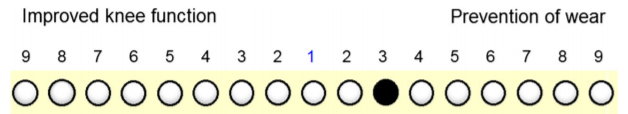
\includegraphics[width=0.75\linewidth]{Figures/AHP1.PNG}
    \captionsetup{justification=centering}
    \caption{Example of an AHP ranking of criteria \cite{AHPtut}}
    \label{AHP1}
\end{figure}

With $n$ criteria, a $n \times n$ matrix is created where the relative importance is shown. The rows are then multiplied and the $n^\text{th}$ root is taken, to normalise the values. In \autoref{AHP}, an example of a trade-off table using AHP is shown. It can be seen in the first row that time and work are considered respectively 3 and 6 times as important as the location. In the final column, the normalised priorities are placed, showing work as the main priority. These values can now be used as weighting factors, which are then multiplied by the quantitative values of each criterion. 

\begin{table}[H]
    \centering
    \captionsetup{justification=centering}
    \caption{Example of an AHP table to determine criteria weights \cite{AHP}} \vspace{-0.2cm}
    \label{AHP}
    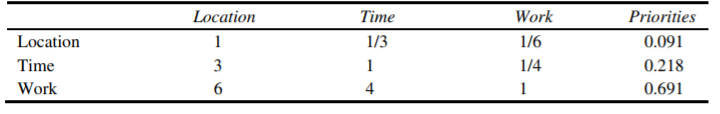
\includegraphics[width=0.75\linewidth]{Figures/AHP.PNG}
\end{table}

The advantage of AHP is that it is a repeatable technique, which is capable of comparing detailed and complex systems. However, the results should not be considered as exact as they seem. A sensitivity analysis on the weights will will also be performed to observe the differences in trade-off outcome \cite{tradeoff}. 

\section{Weights}
\label{subsec:weights}
Two trade-offs will be performed in order to choose a winner from our pool of concepts. First, the different concepts for every capacity range are traded-off based on only quantitative criteria. Thereafter, the winning concepts will be traded-off based on both quantitative and qualitative criteria. The weights factors for both trade-offs are determined in a similar manner, as was described in \autoref{AHPMethod}. For both trade-offs, a digital form was created where group members would first score the main criteria, followed by scoring the sub-criteria. The group members were asked to fill the form individually to prevent any bias. The local weights of the sub-criteria were multiplied by the weights of the main criteria to get the final weight.

In \autoref{AHPtable} the weight factors for the trade-off are shown. The third column consists the weights of the quantitative criteria that are used during the intermediate trade-off. The weights for the final trade-off, including the qualitative criteria, are shown in the fourth column of the trade-off.


%In bll be used during the second trade-offoth tables, the individual weights resemble the weights of the sub-criteria compared to each other. These individual weights are then multiplied with the weights of the main criteria to find the total weight of each sub criterion.

% % Please add the following required packages to your document preamble:
% % \usepackage{multirow}
% \begin{table}[h]
% \captionsetup{justification=centering}
% \caption{Weights of the quantitative criteria and sub-criteria}
% \label{Quanttable}
% \begin{tabular}{|l|l|c|c|}
% \hline
% \multicolumn{1}{|c|}{\textbf{Criteria (weight)}} & \textbf{Sub-criteria} & \textbf{Inividual weight} & \textbf{Total weight} \\ \hline
% \multirow{2}{*}{\textbf{\begin{tabular}[c]{@{}l@{}}Ecological Sustainability\\ (0.36)\end{tabular}}} & Energy demand/hour & 0.781 & 0.278 \\ \cline{2-4} 
%  & Battery mass & 0.219 & 0.078 \\ \hline
% \multirow{2}{*}{\textbf{\begin{tabular}[c]{@{}l@{}}Social Acceptance\\ (0.31)\end{tabular}}} & Noise & 0.825 & 0.258 \\ \cline{2-4} 
%  & Downwash & 0.175 & 0.055 \\ \hline
% \textbf{\begin{tabular}[c]{@{}l@{}}Cost/Profit (0.19)\end{tabular}} & Ticket price & 0.189 & 0.189 \\ \hline
% \textbf{\begin{tabular}[c]{@{}l@{}}Technical Risk (0.14)\end{tabular}} & ATM/UTM efforts & 0.142 & 0.142 \\ \hline
% \end{tabular}
% \end{table}

\begin{table}[H]
\captionsetup{justification=centering}
\caption{Weights of the criteria and sub-criteria}
\label{AHPtable}
\resizebox{\textwidth}{!}{%
\begin{tabular}{|l|l|c|c|}
\hline
\multicolumn{1}{|c|}{\textbf{Criteria (weight)}}      & \multicolumn{1}{c|}{\textbf{Sub-criteria}} & \textbf{Intermediate trade-off}     & \textbf{Final trade-off}    \\ \hline
\multirow{2}{*}{\textbf{\begin{tabular}[l]{@{}l@{}}Ecological Sustainability\\ (0.36)\end{tabular}}} & Energy demand/hour                & 0.278                 & 0.278                 \\ \cline{2-4} 
                                                                                        & Battery mass  & 0.078                 & 0.078  \\ \hline
\multirow{4}{*}{\textbf{\begin{tabular}[l]{@{}l@{}}Social Acceptance \\ (0.31)\end{tabular}}} & Safety               &            -           & 0.185                      \\ \cline{2-4} 
                                                                                       & Passenger experience &           -            & 0.056                      \\ \cline{2-4} 
                                                                                       & Noise                & 0.258                      & 0.055                      \\ \cline{2-4} 
                                                                                       & Downwash             & 0.055 & 0.017 \\ \hline
\multirow{2}{*}{\textbf{\begin{tabular}[l]{@{}l@{}}Cost/Profit \\ (0.19)\end{tabular}}} & Development cost &        -      & 0.036                 \\ \cline{2-4} 
                             & Ticket price  & 0.189                 & 0.153                               \\ \hline
\multirow{3}{*}{\textbf{\begin{tabular}[l]{@{}l@{}}Technical Risk\\ (0.14)\end{tabular}}} & ATM/UTM efforts                      & 0.142                 & 0.081                 \\ \cline{2-4} 
                                                                                         & Susceptibility to weather conditions &         -         & 0.043                 \\ \cline{2-4} 
                                                                                          & Modification of regulations          &      -            & 0.018                 \\ \hline
\end{tabular}%
}
\end{table}
A Consistency Ratio (CR) is computed to ensure that no contradictions occur in the pairwise criteria. This number checks if the scores given to the pairwise comparisons relate logically with each other. It essentially compares the weights generated by the team to a random distribution of the weights. The CR should have a value below $0.10$ for the weight determination to be considered acceptable \cite{AHPtut}. The CR values for all the weight determinations were found to be smaller than $0.10$. This indicates that the pairwise comparisons do not have to be revised. A more detailed explanation of the process used to determine the CR is given in \cite{greenAHP}. 



